\documentclass[12pt]{article}
\usepackage{graphicx}
\usepackage{amsmath}
\usepackage{siunitx}
\usepackage{float}
\graphicspath{ {./images/} }


\title{\huge{Sensors, Measurements \& Instrumentation Assignment II}}
\author{\huge{Papa Kofi Boahen}}
\date{\today} 

\begin{document}
\maketitle
\huge{Roll Number: 10211100334} \par  BSc Computer Engineering
	
\section*{Question 1}
\begin{figure}[H]
	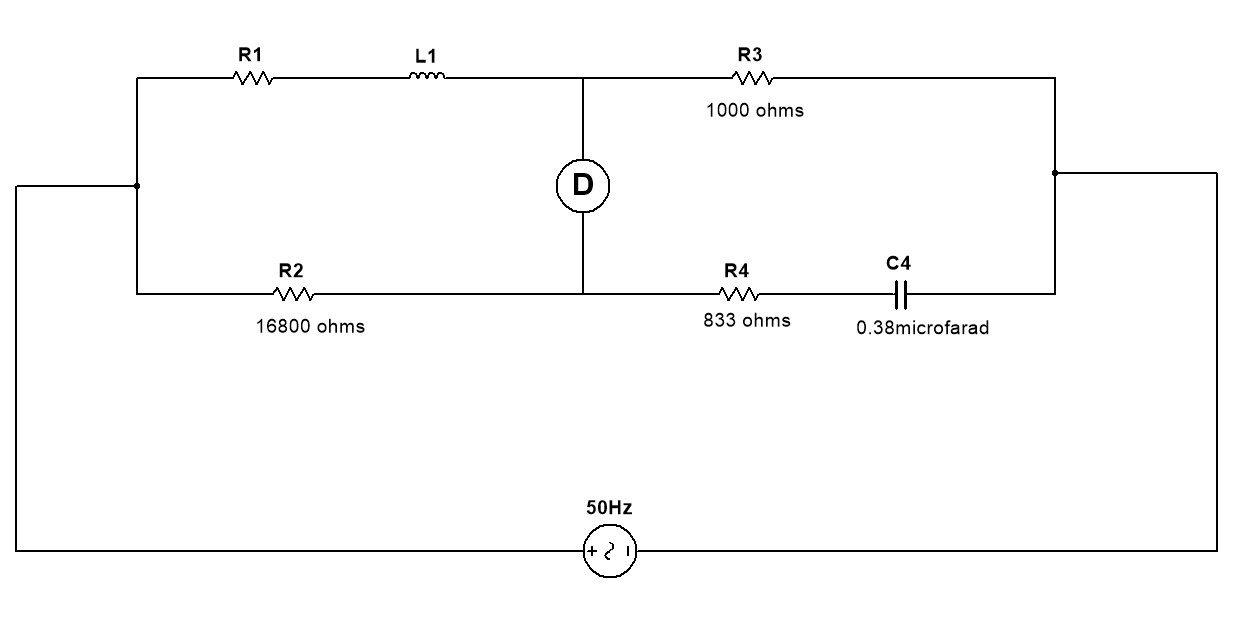
\includegraphics[width=\textwidth]{number1}
\end{figure}

\begin{align*}
	I) \qquad	
		L_{1} &= \frac{R_2R_3C_4}{1+\omega^2R_4^2C_4^2} \\
		\\
	L_{1} &= \frac{(16800)(1000)(\num{0.38e-6})} {1+(314.2)^2(833)^2 (\num{0.38e-6})^{2}} \\
	L_{1} &= \underline{\underline{\qty{6.32}{\henry}}}
\end{align*}

\vspace{2cm}

\begin{gather*}
	II) \qquad	
	R_{1} = \frac{\omega^2C_4^2R_2R_3R_4}{1+\omega^2R_4^2C_4^2} \\
	\\
	R_{1} = \frac{(314.2)^2(\num{0.38e-6})^2(16800)(1000)(833)} {1+(314.2)^2(833)^2 (\num{0.38e-6})^{2}} \\
	\\
	R_{1} = \underline{\underline{\qty{197}{\ohm}}}
\end{gather*}

\section*{Question 2}
\begin{figure}[H]
	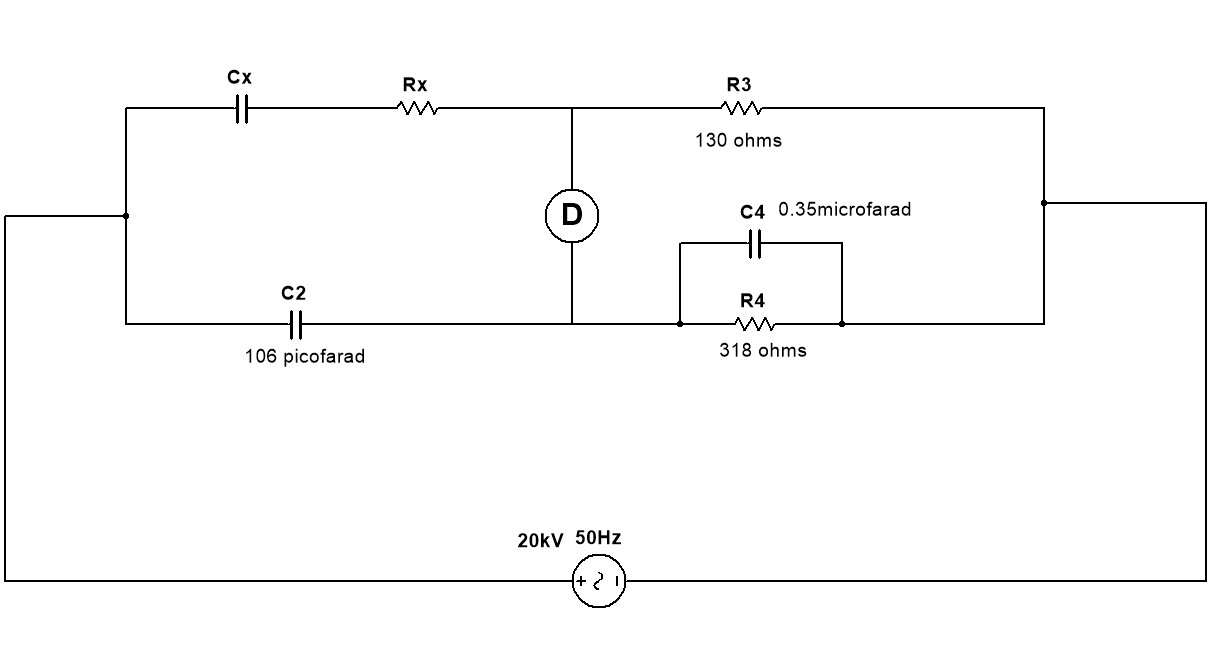
\includegraphics[width=\textwidth]{number2}
\end{figure}

I) \quad \[{{\text{Z}}_{\text{x}}}{{\text{Z}}_{\text{4}}}\text{ = }{{\text{Z}}_{\text{2}}}{{\text{Z}}_{\text{3}}} \]

\[ {{\text{R}}_{\text{x}}}{{\text{R}}_{\text{4}}}\text{+ }\frac{1}{\text{j}\omega {{\text{C}}_{\text{x}}}}{{\text{R}}_{\text{4}}}\text{ = }\!\!~\!\!\text{  }\frac{{{\text{R}}_{\text{3}}}}{\text{j}\omega {{\text{C}}_{\text{2}}}}\text{+}\frac{\text{j}\omega {{\text{C}}_{\text{4}}}{{\text{R}}_{\text{4}}}{{\text{R}}_{\text{3}}}}{\text{j}\omega {{\text{C}}_{\text{2}}}}..(1) 
	\]
Since,
 \[\left( \frac{\text{1}}{\text{j}}=-\text{j} \right) \]
Equation 1 can be written as,
\[{{\text{R}}_{\text{x}}}{{\text{R}}_{\text{4}}}-\frac{\text{j}{{\text{R}}_{\text{4}}}}{\omega {{\text{C}}_{\text{x}}}}=-\frac{\text{j}{{\text{R}}_{\text{3}}}}{\omega {{\text{C}}_{\text{2}}}}\text{+}\frac{{{\text{C}}_{\text{4}}}{{\text{R}}_{\text{4}}}{{\text{R}}_{\text{3}}}}{{{\text{C}}_{\text{2}}}}\]

Now equating real terms,
\[{{\text{R}}_{\text{x}}}{{\text{R}}_{\text{4}}}=\frac{{{\text{C}}_{\text{4}}}{{\text{R}}_{\text{4}}}{{\text{R}}_{\text{3}}}}{{{\text{C}}_{\text{2}}}} \]

\[ {{\text{R}}_{\text{x}}}=\frac{{{\text{R}}_{\text{3}}}{{\text{C}}_{\text{4}}}}{{{\text{C}}_{\text{2}}}} \]

Equating imaginary terms,
\[ -\frac{\text{j}{{\text{R}}_{\text{4}}}}{\omega {{\text{C}}_{\text{x}}}}=-\frac{\text{j}{{\text{R}}_{\text{3}}}}{\omega {{\text{C}}_{\text{2}}}}\]

Expression for $C_x$, 
\[ C_{x} = \frac{R_{4}C_{2}}{R_{3}} \]

\begin{align*}
	II) \qquad	
	C_{x} &= \frac{R_4C_2}{R_3} \\
	C_{x} &= \frac{318\times\num{106e-12}}{130} \\
	C_{x} &= \underline{\underline{\qty{259.29}{\pico\farad}}}
\end{align*}

\vspace{2cm}

\begin{align*}
	III) \qquad	
	R_{x} &= \frac{R_3C_4}{C_2} \\
	R_{x} &= \frac{130\times\num{0.35e-6}}{\num{106e-12}} \\
	R_{x} &= \underline{\underline{\qty{429.25}{\kilo\ohm}}}
\end{align*}

\section*{\underline{Precautions}}
I) Ensure the voltage does not exceed 5V. \\
II) Ensure tight connections.

\vspace{1cm}

\begin{gather*}
IV) \quad	
Power factor, pf = \omega C_{x}R_{x} \\
= 2\times\pi\times50\times\num{259.29e-12}\times\num{429.25e3} \\
= \underline{\underline{0.0345}}
\end{gather*}	

\vspace{2cm}	 

\section*{Question 3}
\begin{figure}[H]
	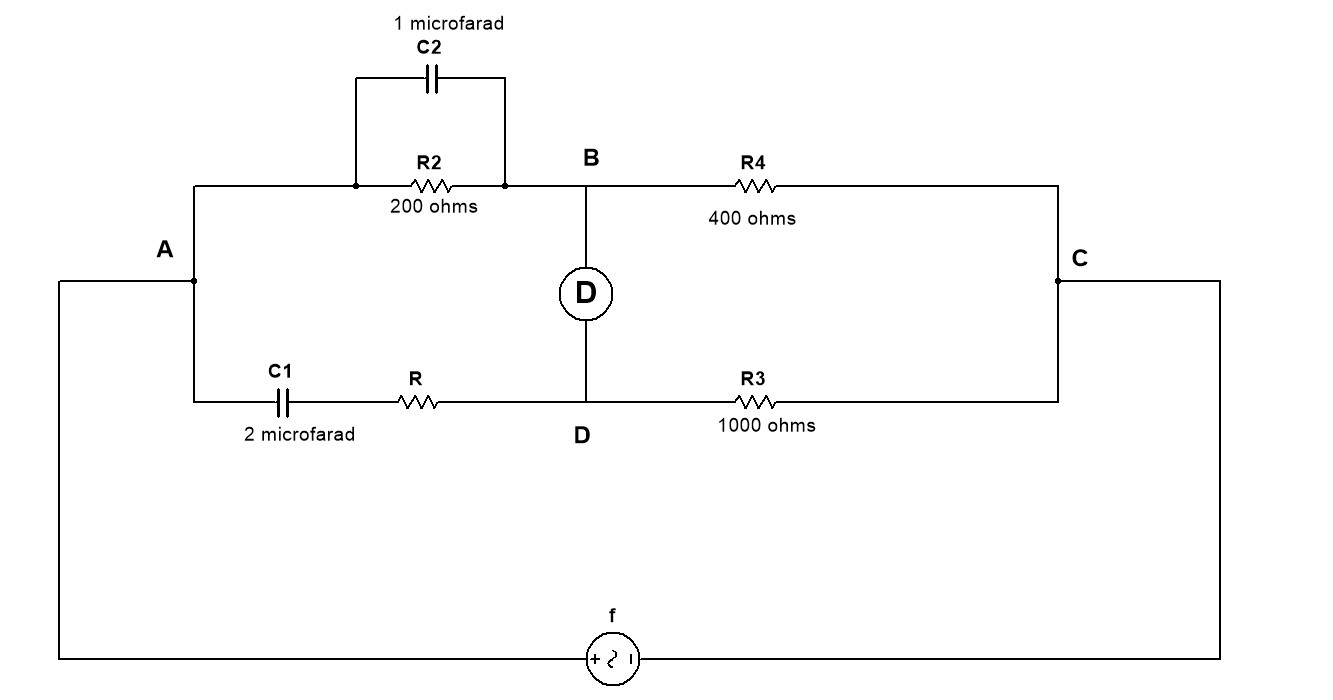
\includegraphics[width=\textwidth]{number3a}
\end{figure}

Parallel Wein's Bridge,
\begin{align*}
I) \quad\frac{C_2}{C_1} &= \frac{R_3}{R_4} - \frac{R}{R_2} \\
\frac{\num{1e-6}}{\num{2e-6}} &= \frac{1000}{400}-\frac{R}{200} \\
R &= \frac{1600}{4} \\
R  &= \underline{\underline{\qty{400}{\ohm}}}
\end{align*}

\begin{align*}
II) \quad f &= \frac{1}{2\pi\sqrt{RR_2C_1C_2}} \\
			&= \frac{1}{2\pi\sqrt{400\times200\times\num{1e-6}\times\num{2e-6}}} \\
			&= \underline{\underline{\qty{397.89}{\hertz}}}
\end{align*}

\vspace{2cm}
\section*{Question 4}
\textbf{The question given did not have a preamble, incomplete question given.}

\section*{Question 5}
\begin{figure}[H]
	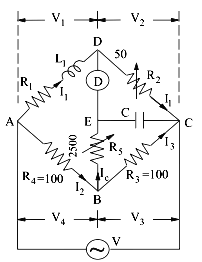
\includegraphics[width=\textwidth]{ac5}
\end{figure}

\begin{align*}
I)\quad	R_1 &= R_2\left(\frac{R_4}{R_3}\right) \\
	    &= 50 \times \left(\frac{100}{100} \right) \\
	    &= \underline{\underline{\qty{50}{\ohm}}}
\end{align*}

\begin{multline*}
II) \quad	L_1 = C\frac{R_2}{R_3}\times\left[R_5(R_4+R_3)+R_4R_3\right] \\
= \num{1e-6}\times\frac{50}{100}\left[2500(100+100)+(100\times100)\right] \\
L_1 = \underline{\underline{\qty{0.255}{\henry}}}
\end{multline*}
	




\end{document}